\documentclass[12pt]{article}
\usepackage{fullpage,epsfig,latexsym}
\setlength{\headsep}{.4in}
\parskip 6pt
\def\Six{{\sc Six}}
\def\Mg{{\sc Mongoose}}

\begin{document}
\pagestyle{plain}

\vspace*{-.5in}
{\it to appear in ICGA Journal}
\vspace*{.5in}

\begin{center}
{\large\bf Hex Gold at Graz: Six defeats Mongoose} \\ \ \\
{\bf G{\'a}bor Melis\footnote{mega@hotpop.com, http://six.retes.hu/} and
     Ryan Hayward\footnote{Department 
       of Computing Science, 
       University of Alberta, Edmonton Canada,
       hayward@cs.ualberta.ca,
       http://www.cs.ualberta.ca/$\sim$hayward.
       The support of NSERC and 
       the UofA GAMES group is gratefully acknowledged.}
}
\end{center}

{\noindent\large\bf The contestants.}
2003 saw a Hex tournament take place at the Computer Games Olympiad 
for the first time since 1999, when 
Vadim Anshelevich's {\sc Hexy} (gold) defeated 
Jack van Rijswijck's {\sc Queenbee} (silver) and 
Emanuel Brasa's {\sc KillerBee} (bronze) \cite{Ansh00b}.

This year's tournament had two new entrants:
\Six\ by G{\'a}bor Melis, and
\Mg\ by Yngvi Bjornsson, Ryan Hayward, Mike Johanson, 
Morgan Kan, and Nathan Po.
Both programs incorporate the key ideas behind Hexy \cite{Ansh02},
finding virtual connections via H-search 
(which uses {\sc and} and {\sc or} composition rules)
and then computing an edge-to-edge resistance measure 
based on which pairs of cells are virtually connected.

\Six\ performs a 2-ply search with alpha-beta pruning,
analysing the most promising 20 1-ply and 15 2-ply moves.
With a game tree search this shallow,
most of the work is done within the H-search. 
\Six's implementation of H-search keeps track of all computed virtual
connections and virtual semi-connections between groups, 
but uses only a small number of them, 
namely those with the smallest carriers
(the carrier of a virtual connection is the associated
set of empty cells which guarantees the connection). 
The feature which most contributes to 
\Six's characteristic style of play is the computation 
of connections which go through the edge of the board,
namely connections which can only be constructed 
by using one of the board edges as the pivot point in the {\sc and} rule.
\Six\ does not have an opening book.
During the opening four moves of the game, 
it dispenses with 2-ply altogether and
considers only 30 1-ply moves,
although with an H-search which is more thorough than usual.
The \Six\ source code can be freely downloaded from
http://hex.retes.hu/six.

\Mg\ uses alpha-beta search with iterative deepening,
searching as deeply as the allocated time for a given move permits.
For opening play, it uses a book for the first two to four moves,
depending on the position.
A characteristic feature of \Mg\ is its move pruning.
As described in \cite{HB03}, it reduces the number of moves 
under consideration by in some cases
deducing that a move is provably inferior to some other move,
and in other cases determining
that one or more stones can be added to the board
without changing the theoretical outcome of the game.

\begin{figure}\label{fig1}
\epsfig{file=g1.eps,height=150pt,width=245pt}
\hspace*{-.2in}\epsfig{file=g2.eps,height=150pt,width=245pt}
\caption{Games 1 and 2.
In Game 1, \Six\ (black) opens with 1.A3 and wins quickly.
In Game 2, \Mg\ opens with 1.B3, \Six\ swaps (black), and \Six\ wins again.}
\end{figure}

{\noindent\large\bf Double-round 1.}
The first \Six/\Mg\ double-round of four games (Figures 1 and 2)
started in the Graz Casino on Sunday November 23 at 14:00.
\Six\ (black) opened Game 1 with 1.A3
and won quickly after questionable early moves 6.H5 and 10.E5 by \Mg.
\Mg\ opened Game 2 with 1.B3 and \Six\ swapped (taking black).
Again, \Six\ won quickly after some suspect early \Mg\ moves,
namely 5.E8, 7.F9, and 9.G10.
\Six\ (black) also  won Game 3 quickly.
Game 4 was the longest and most interesting game of the double-round,
but the outcome was the same, 
with \Six\ (white) winning to take a 4-0 lead.

{\noindent\large\bf The interlude.}
After Double-round 1, the players retired to a restaurant 
to sample some local cuisine and analyse the games thus far.
{\sc Queenbee} had also registered for the tournament,
so \Six\ and \Mg\ were not scheduled to play any further games 
against each other.
For this reason, the after-dinner discussion was open and enlightening.
In particular, it emerged that \Mg's weak early play
was likely a result of the odd/even-ply search effect:
in Hex as in many other board games,
position evaluations after a player's move are 
usually more optimistic than after an opponent's move.

This analysis came into play the next day,
when {\sc Queenbee} withdrew from the tournament due to illness.
To complete the tournament, \Six\ and \Mg\ were
required to play a second double-round.

{\noindent\large\bf Double-round 2.}
The second and final \Six/\Mg\ double-round of four games (Figures 3 and 4)
took place in the Graz casino on Monday November 24.
In Game 5, in order to avoid any weak 3-ply moves,
\Mg\ changed settings and restricted the search depth to 2-ply for the first 10 moves.
The result was \Mg's first win,
and the sudden injection of some drama into the  competition,
which to this point had been decidedly one-sided.
In Game 6, \Mg\ seemed on the road to a second consecutive victory,
with a strong ladder under construction in the middle game.
But then the odd/even-ply gremlin struck \Mg\ again,
when a 3-ply search selected 29.J8 over the 2-ply selection 29.F2.
This blunder allowed \Six\ (black) to break the ladder with 30.F2
and win the game soon after.
For the remaining two games, \Mg\ played with search
depth restricted to 2-ply,
but the damage was done: \Six\ had a 5-1 lead and the gold medal.

\begin{figure}\label{fig2}
\epsfig{file=g3.eps,height=150pt,width=245pt}
\hspace*{-.2in}\epsfig{file=g4.eps,height=150pt,width=245pt}
\caption{Games 3 and 4.
\Six\ (black) wins Game 3, with the \Mg\ operator resigning after 27.B3.
In Game 4 \Mg\ puts up a better fight, but \Six\ (white) wins again.}
\end{figure}

In Game 7,
having already won the championship, \Six\ decided to play an opening
which would almost never be played in a tournament: 1.C5 is so strong
that the opponent will probably swap and win easily.
This was indeed what happened. \Mg\ swapped (taking black) and went
on to win, but not before \Six\ put up a good fight.
\Six's 3.E7 was strong: on the short diagonal
and only one cell from the center, it thwarts the threat from C5.
Black then moved to reduce White's options, with 4.C8 forcing 5.C7.
After 10.A9 11.B9 12.B8, White found itself in a bad position,
with the upper part of the board cut off and 
a ladder forming on row eight. 
Black played a satisfactory ladder escape with 16.I7,
and from that point all White could do was to delay the inevitable:
the black stone at I7 was virtually connected to the lower edge,
and once the possibility of a direct connection to the upper edge was lost,
it simply steered back towards the black pieces at C5 and D7,
eventually breaking through to the upper edge with 58.D4.

In Game 8, \Mg\ returned the favour offered by \Six\
in the previous game and opened with 1.C5. 
As expected, \Six\ swapped (taking black) and won.
\Six's victory was quicker than in the previous game.
After the swap, \Mg\ played the rather weak 3.C9,
which after 4.F7 left Black with a huge advantage. 
While 5.F6 seemed to be a reasonable attempt to cut off F7 from the upper edge,
it was unlikely to succeed, as C5 was well placed to assist F7.
5.F8 might have been stronger. 
With a forcing escape at B10 available, 
Black had every opportunity to end the game quickly;
instead, Black played quietly,
securing the victory with a succession of positional moves.

{\noindent\large\bf Epilogue.}
While conceptually similar, \Six\ and \Mg\ exhibited different
strengths and weaknesses. Once the odd/even-ply effect was muted,
\Mg\ played a convincing game that at times seemed stronger than what
\Six\ could offer. However, \Six's forte, 
namely its opening and positional play, balanced the scales. 
For board-size 11,
both programs played at a level that is on par with intermediate human players
and clearly below that of human experts.
It will be interesting to see how much progress can be made
before the upcoming July 2004 Olympiad.

{\footnotesize
\begin{trivlist}
\item[] 
{\bf Game 1.} \Six\ vs \Mg\ (2003/11/23, first round of day 1)\\
1.A3 2.F6 3.C7 4.C9 5.D8 6.H5 7.B10 8.C6 9.D6 10.E5
11.D5 12.C8 13.B7 14.B8 15.A8 16.A9 17.E7 18.G7 19.D9
20.C10 21.E6 22.D10 23.F9 24.G10 25.E10 26.E9 27.F8 28.F7
29.E8 30.F5 31.E3 32.H8 33.D4 34.B4 35.D11 36.B3 37.D2
38.A6 39.E2 40.B6 41.F1
Black (\Six) wins.

\begin{figure}\label{fig3}
\epsfig{file=g5.eps,height=150pt,width=245pt} 
\hspace*{-.2in}\epsfig{file=g6.eps,height=150pt,width=245pt}
\caption{Games 5 and 6.
In Game 5, \Mg\ (white) wins for the first time.
In Game 6, \Mg\ blunders with 29.J8 and \Six\ (black) wins.}
\end{figure}

\item[] {\bf Game 2.} \Mg\ vs \Six\ (2003/11/23, first round of day 1)\\
1.B3 2.Swap 3.D7 4.F6 5.E8 6.G7 7.F9 8.H8 9.G10 10.E9
11.G6 12.E7 13.D8 14.F7 15.F8 16.F10 17.G9 18.I9 19.H7
20.G8 21.I8 22.H9 23.H11 24.J10 25.G4 26.E5 27.E4 28.C6
29.F3 30.B5 31.D5 32.D6 33.C5 34.I3 35.I4 36.B6 37.J9
38.I10 39.B4 40.C4 41.J3 42.D2 43.H6 44.C3 45.B9 46.D1
47.A9 48.E6 49.B1 50.I11
Black (after swapping) (\Six) wins.

\item[] {\bf Game 3.} \Six\ vs \Mg\ (2003/11/23, second round of day 1)\\
1.A2 2.H5 3.E6 4.E5 5.F5 6.F3 7.G3 8.C8 9.D8 10.D7
11.E7 12.D9 13.E10 14.C6 15.C9 16.J4 17.D10 18.D4 19.C10
20.I7 21.F4 22.H1 23.I2 24.G8 25.H2 26.I3 27.B3
Black (\Six) wins.

\item[] {\bf Game 4.} \Mg\ vs \Six\ (2003/11/23, second round of day 1)\\
1.B6 2.F6 3.C8 4.C7 5.E7 6.E6 7.A8 8.B7 9.A7 10.B8
11.A9 12.C5 13.D6 14.D7 15.K4 16.B10 17.B9 18.D9 19.C10
20.C9 21.F8 22.I3 23.D8 24.F7 25.E8 26.B5 27.C6 28.E4 29.E5
30.F4 31.H4 32.H3 33.G4 34.G3 35.K2 36.K1 37.J2 38.J1 39.I2
40.I1 41.H2 42.H1 43.D4 44.F2 45.G2 46.G1 47.E3 48.D5 49.F3
50.J4 51.I4 52.J3 53.K3 54.J5 55.K5 56.E2 57.C3 58.C4 59.D3
60.D1 61.B2 62.B3 63.C2 64.B1 65.C1 66.J6 67.K6 68.J7 69.K7
70.J9 71.J8 72.I9 73.I8 74.H9 75.H8 76.G9 77.E10 78.G8
79.H7 80.G7 81.H5 82.F5 83.A6 84.B4 85.A4 86.A5 87.I5 88.K9
White (\Six) Wins.

\item[] {\bf Game 5.} \Six\ vs \Mg\ (2003/11/24, first round of day 2)\\
1.A2 2.F6 3.C7 4.C8 5.G6 6.F8 7.E8 8.D7 9.B9 10.C9
11.I5 12.I3 13.K2 14.J4 15.I4 16.H7 17.F7 18.G4 19.F5
20.D10 21.E9 22.E10 23.C10 24.D9 25.B10 26.B8 27.F9 28.J3
29.H3 30.H4 31.G5 32.F4 33.E5 34.E4 35.D5 36.D4 37.K3
38.K4 39.B5 40.C5 41.A6 42.B6 43.A8 44.A7
White (\Mg) wins.

\item[] {\bf Game 6.} \Mg\ vs \Six\ (2003/11/24, first round of day 2)\\
1.A2 2.F6 3.G6 4.G5 5.I4 6.I3 7.K2 8.J3 9.H4 10.H3
11.G4 12.G3 13.K3 14.J4 15.K4 16.J5 17.K5 18.J6 19.K6 20.K1
21.J2 22.J1 23.I2 24.I1 25.H2 26.H1 27.G2 28.G1 29.J8 30.F2
31.F3 32.E3 33.C4 34.B3 35.B6 36.D2 37.E4 38.C2 39.C6 40.A3
41.A6 42.E2 White (\Six) wins.

\item[] {\bf Game 7.} \Six\ vs \Mg\ (2003/11/24, second round of day 2)\\
1.C5 2.Swap 3.E7 4.C8 5.C7 6.D7 7.C9 8.D8 9.D9 10.A9
11.B9 12.B8 13.A10 14.E8 15.E9 16.I7 17.G8 18.F8 19.F9
20.H9 21.I8 22.J7 23.H8 24.J8 25.I10 26.I9 27.G11 28.F10
29.E11 30.F11 31.H6 32.G7 33.H7 34.I5 35.I6 36.K5 37.K6
38.J6 39.G9 40.G10 41.J5 42.K4 43.J3 44.J4 45.H4 46.I3
47.I4 48.H5 49.G6 50.G5 51.G4 52.F6 53.E6 54.F5 55.F4
56.E5 57.E2 58.D4 59.C3 60.F3 61.H1 62.F2 63.F1 64.G1
65.B6 66.E4
Black (after swapping) (\Mg) wins.

\begin{figure}\label{fig4}
\epsfig{file=g7.eps,height=150pt,width=245pt}
\hspace*{-.2in}\epsfig{file=g8.eps,height=150pt,width=245pt}
\caption{Games 7 and 8.
\Six\ opens Game 7 with 1.C5; \Mg\ swaps (black) and wins.
\Mg\ opens Game 8 with 1.C5;
\Six\ swaps (black) and wins.
\Six\ defeats \Mg\ 6-2.}
\end{figure}

\item[] {\bf Game 8.} \Mg\ vs \Six\ (2003/11/24, second round of day 2) \\
1.C5 2.Swap 3.C9 4.F7 5.F6 6.H5 7.H4 8.G5 9.G3 10.G4
11.I2 12.E5 13.F4 14.J2 15.I3 16.J3 17.I4 18.I5 19.J4 20.D7
21.E7 22.D8 23.D9 24.E8 25.D6 26.E4 27.E9 28.F9 29.F8 30.H7
31.I6 32.G7 33.D4 34.E3 35.E2 36.D3 37.D2 38.F2 39.G9 40.G8
41.B8 42.F10 43.B3 44.E11 45.B5 46.E6 47.B6 48.G1
Black (after swapping) (\Six) wins.
\end{trivlist}
}

\bibliographystyle{plain}
\bibliography{rpt}
\end{document}
